\appendix 

\addtocontents{toc}{\protect\setcounter{tocdepth}{1}}

\chapter{Anhang} 

%%%%%%%%%%%%%%%%%%%%%%%%%%%%%%%%%%%%%%%%%%%%%%%%%%%%%%%%%%%%%%%%%%%
\section{Verweise}                    %%%%%%%%%%%%%%%%%%%%%%%%%%%%%
%%%%%%%%%%%%%%%%%%%%%%%%%%%%%%%%%%%%%%%%%%%%%%%%%%%%%%%%%%%%%%%%%%%


%%%%% Plot der Auszahlungsfunktion der Optionen %%%%%%%%%%%%%%%%%%%%%%%%%%%%%%%%%%%
\subsection{Plot der Auszahlungsfunktionen \ref{GL:payoffCall} und \ref{GL:payoffPut} \label{Anhang:PlotPayoff}}
\begin{figure}[h]
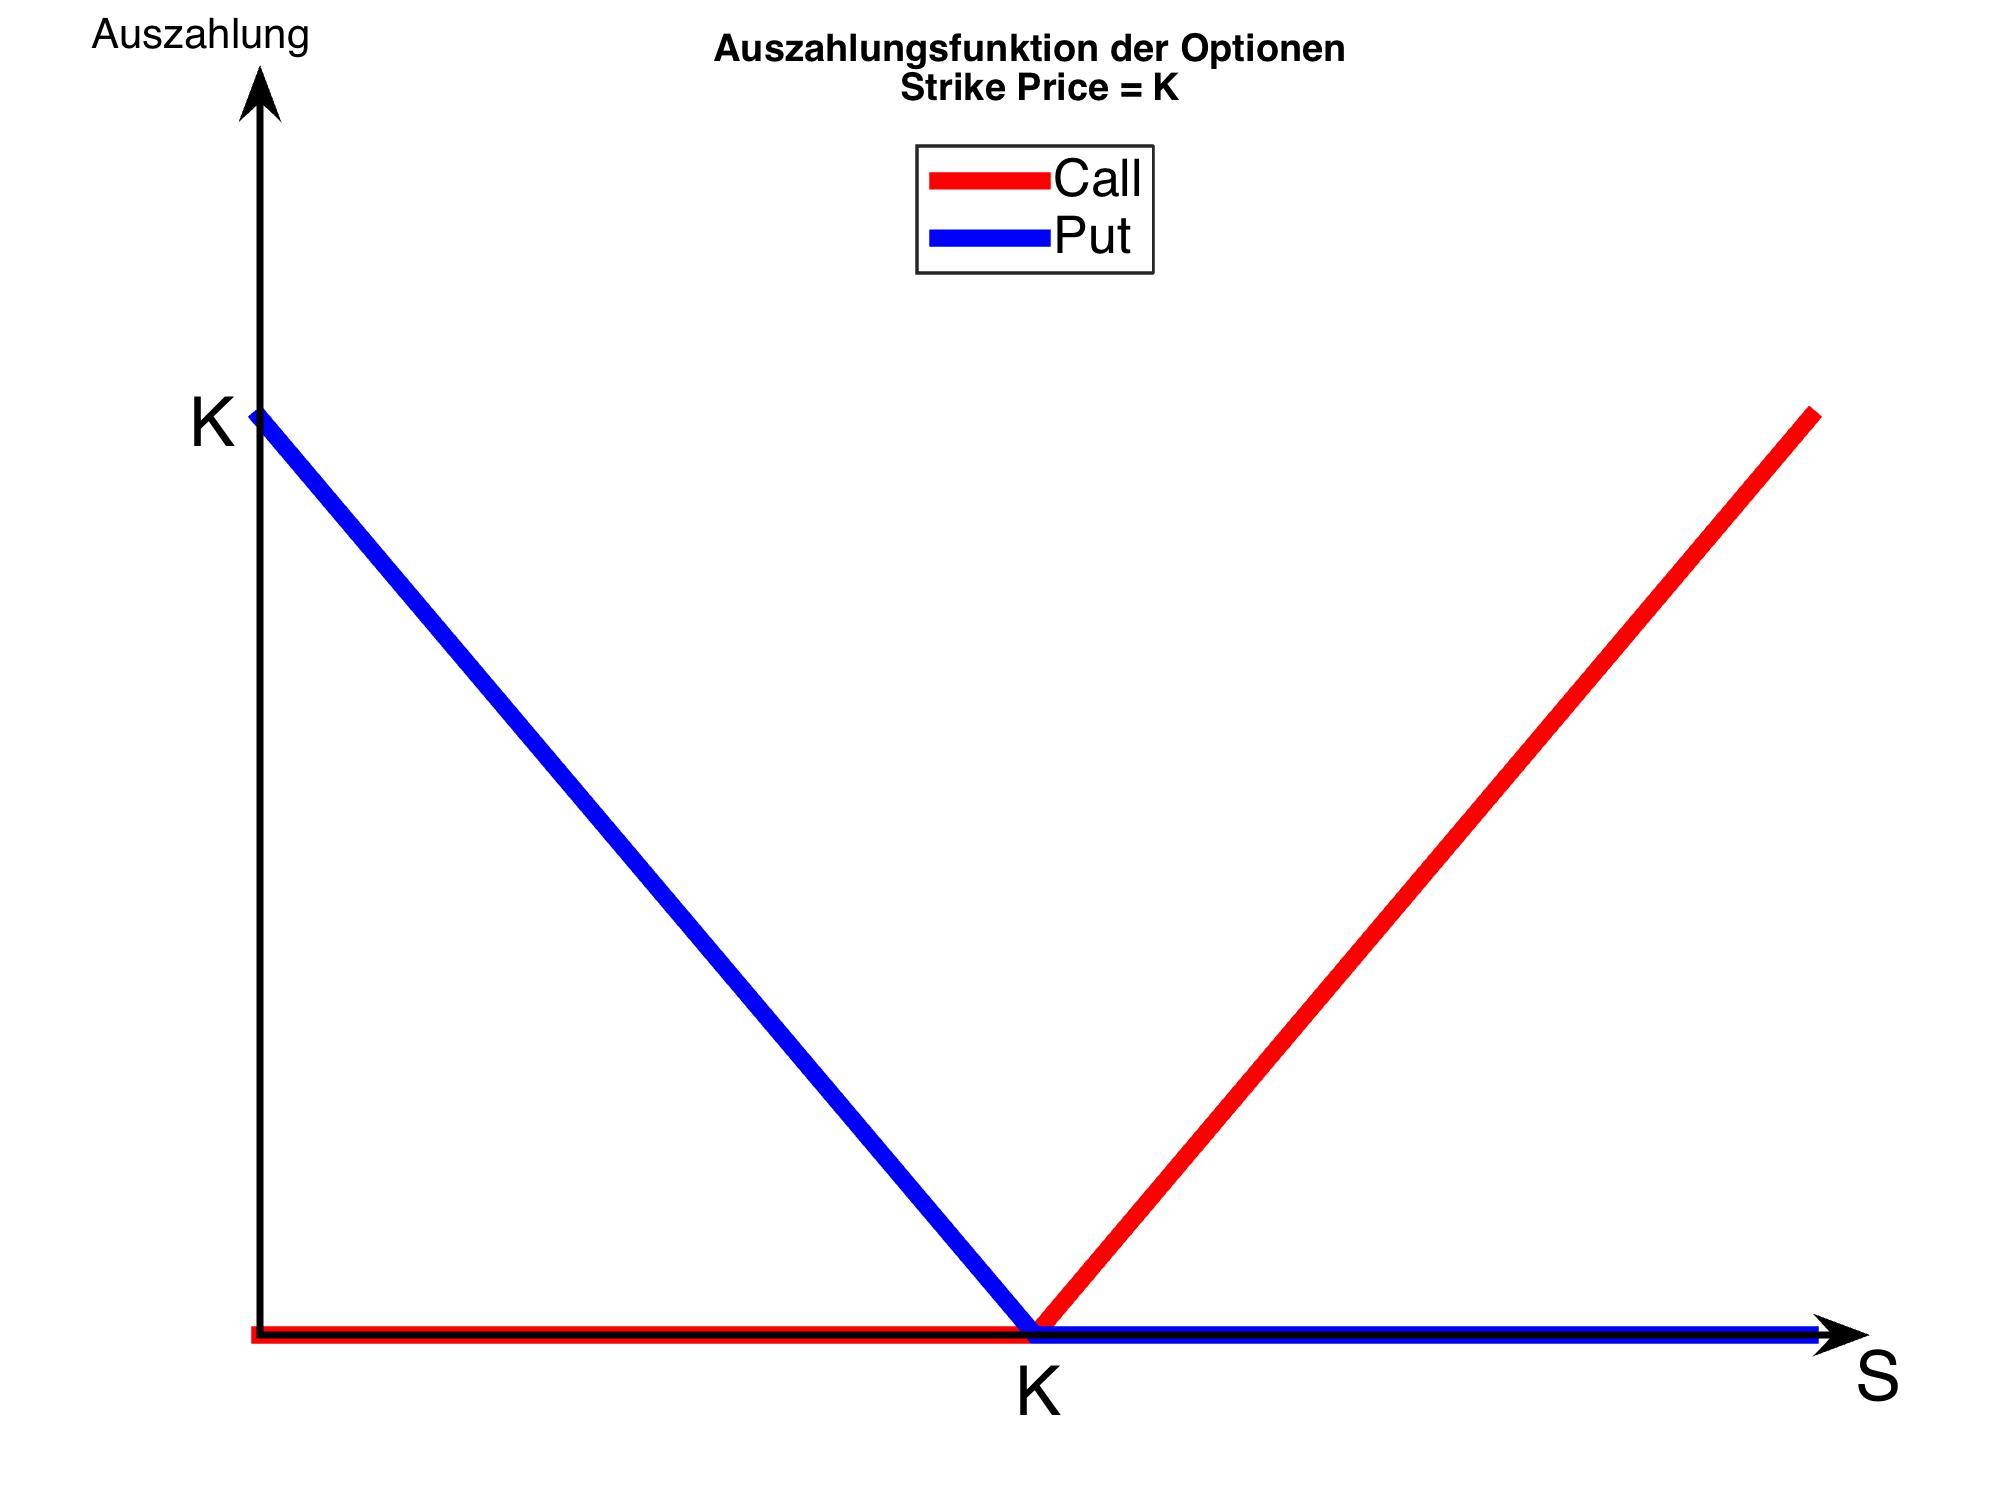
\includegraphics[width=1\textwidth]{PayoffOptionen.jpg}
\caption{Auszahlungsfunktionen einer Call- und Put-Option}
\end{figure}


%%%%% Lösung des Gleichungssystems der Duplikationsstrategie %%%%%%%%%%%%%%%%%%%%%%
\subsection{Lösung des Gleichungssystems \ref{Bin:gleichungssystem} }
\label{Anhang:LGS}
In Matrixform geschrieben ergibt sich aus (\ref{Bin:gleichungssystem}):
\begin{equation*} \begin{pmatrix}
    e^{r\Delta t} & uS \\
    e^{r\Delta t} & dS \\
\end{pmatrix} 
\begin{pmatrix}
    c_1 \\
    c_2 \\
\end{pmatrix} = 
\begin{pmatrix}
    C_u \\
    C_d \\
\end{pmatrix}
\end{equation*}
Dessen Lösung sich ergibt als
\begin{equation*}
\begin{pmatrix}
    c_1 \\
    c_2 \\
\end{pmatrix} =
\frac{1}{e^{r\Delta t}S\left(d-u\right)}
\begin{pmatrix}
    dS &  -uS \\
    -e^{r\Delta t} & e^{r\Delta t} \\
\end{pmatrix}
\begin{pmatrix}
    C_u \\
    C_d \\
\end{pmatrix} = 
\begin{pmatrix}
\frac{S\left(dC_u - uC_d\right)}{e^{r\Delta t}S\left(d-u\right)} \\
\frac{e^{r\Delta t}\left(C_d-C_u\right)}{e^{r\Delta t}S\left(d-u\right)}
\end{pmatrix}=
\begin{pmatrix}
    \frac{uC_d - dC_u}{e^{r\Delta t}(u-d)} \\
    \frac{C_u - C_d}{S(u-d)} \\
\end{pmatrix}
\end{equation*}

%%%%%%%%%%% Lösung des Gleichungssystems für die neue Wahl der Parameter %%%%%%%%%%%%%%
\subsection{Lösung des Gleichungssystems (\ref{BIN:GS1})-(\ref{BIN:GS2})}
\label{Anhang:GSParameter}

Auflösen von (\ref{BIN:GS1}) nach $p$ liefert:
\begin{equation*}
p = \frac{\left(r-\frac{1}{2}\sigma^2\right)\Delta t - ln(d)}{ln\left(\frac{u}{d}\right)}
\end{equation*}
Mit der Zusatzbedingung $d = \nicefrac{1}{u}$ und Einsetzen in (\ref{BIN:GS2}) folgt:
\begin{eqnarray*}
\sigma^2\Delta t & = & ln\left(\frac{u}{d}\right)^2\frac{\left(r-\frac{1}{2}\sigma^2\right)\Delta t - ln(d)}{ln\left(\frac{u}{d}\right)}\left(\frac{ln\left(\frac{u}{d}\right)-\left(r-\frac{1}{2}\sigma^2\right)\Delta t + ln(d)}{ln\left(\frac{u}{d}\right)}\right) \\
& = & \left(\left(r-\frac{1}{2}\sigma^2\right)\Delta t - ln(d)\right)\left(ln(u) - \left(r-\frac{1}{2}\sigma^2\right)\Delta t\right) \\
& = & -ln(u)ln(d) - \left(r-\frac{1}{2}\sigma^2\right)(\Delta t)^2 + \underbrace{(ln(u)+ln(d))}_{=0}\left(r-\frac{1}{2}\sigma^2\right)\Delta t \\
& = & ln(u)^2 + \mathcal{O}\left((\Delta t)^2\right)
\end{eqnarray*}
Unter Vernachlässigung des $\left(\Delta t\right)^2$-Termes also
\begin{equation*}
u = e^{\sigma\sqrt{\Delta t}} \text{ und } d = e^{-\sigma\sqrt{\Delta t}}
\end{equation*}
Sowie
\begin{equation*}
p = \frac{\left(r-\frac{1}{2}\sigma^2\right)\Delta t + \sigma\sqrt{\Delta t}}{2\sigma\sqrt{\Delta t}} =\frac{1}{2} + \frac{1}{2}\left(r-\frac{1}{2}\sigma^2\right)\frac{\sqrt{\Delta t}}{\sigma} 
\end{equation*}






%%%%% Taylorentwicklung für altes p %%%%%%%%%%%%%%%%%%%%%% 
\subsection{Wahl des Parameter p in (\ref{BIN:1PeriodenCall}) und (\ref{BIN:parameter})}
\label{Anhang:pundp'}
Sei $p_1 = \frac{e^{r\Delta t} - d}{u-d}$ (aus (\ref{BIN:1PeriodenCall})) und $p_2 = \frac{1}{2} + \frac{1}{2}\left(r-\frac{1}{2}\sigma^2\right)\frac{\sqrt{\Delta t}}{\sigma}$ (aus \ref{BIN:parameter})).
Da $u = e^{\sigma\sqrt{\Delta t}}$ und $d = e^{-\sigma\sqrt{\Delta t}}$, ist $p_1$ eine Funktion von $\Delta t$ und eine Taylorentwicklung liefert:
\begin{eqnarray*}
p_1 & = & \frac{\left(1+r\Delta t\right) - \left(1 - \sigma\sqrt{\Delta t} + \frac{1}{2}\sigma^2\Delta t\right) +  \mathcal{O}\left(\left(\Delta t\right)^{\nicefrac{3}{2}}\right)}{\left(1 + \sigma\sqrt{\Delta t} + \frac{1}{2}\left(\sigma\sqrt{\Delta t}\right)^2\right)- \left(1 - \sigma\sqrt{\Delta t} + \frac{1}{2}\left(\sigma\sqrt{\Delta t}\right)^2\right) + \mathcal{O}\left(\left(\Delta t\right)^{\nicefrac{3}{2}}\right)} \\
  & = & \frac{\sigma + \left(r-\frac{1}{2}\sigma^2\right)\sqrt{\Delta t} +  \mathcal{O}(\Delta t)}{2\sigma + \mathcal{O}(\Delta t)} \\
  %& = & \frac{1}{2 + \mathcal{O}(\Delta t)} + \frac{\left(r-\frac{1}{2}\sigma^2\right)}{2\sigma + \mathcal{O}(\Delta t)} \\
  %& = & \underbrace{\frac{1}{2} + \frac{1}{2}\left(r-\frac{1}{2}\sigma^2\right)\frac{\sqrt{\Delta t}}{\sigma}}_{= p'} +\,\mathcal{O}(\Delta t)
\end{eqnarray*}
Und damit
\begin{equation*}
\lim_{\Delta t \to 0} p_1 =  \lim_{\Delta t \to 0} p_2 = \frac{1}{2} \\
\end{equation*}

%%%%%%%%%%% TAYLORENTWICKLUNG FÜR p'%%%%%%%%%%%%%%%%%%%%%%%%%%%%%%%%%%%%%
\subsection{Grenzwert von $\frac{2p' - 1}{\sqrt{\Delta t}}$ in Satz \ref{BIN:konvergenzCallOption}}
\label{Anhang:Taylorp'} 
Mit $p' = pue^{-r\Delta t}$ gilt:
\begin{eqnarray*}
\frac{2p'-1}{\sqrt{\Delta t}} & = & \frac{2pue^{-r\Delta t}-1}{\sqrt{\Delta t}} \\
 & = & \frac{2\left(\frac{1}{2} + \frac{1}{2}\left(r-\frac{1}{2}\sigma^2\right)\frac{\sqrt{\Delta t}}{\sigma}\right)ue^{-r\Delta t}-1}{\sqrt{\Delta t}} \\
 & = & \left(r-\frac{1}{2}\sigma^2\right)\frac{1}{\sigma}e^{\sigma\sqrt{\Delta t}-r\Delta t} + \frac{e^{\sigma\sqrt{\Delta t}-r\Delta t} - 1}{\sqrt{\Delta t}} \\
 & \overset{\tiny Taylor}{=} & \left(r-\frac{1}{2}\sigma^2\right)\frac{1}{\sigma}\underbrace{e^{\sigma\sqrt{\Delta t}-r\Delta t}}_{\to 1} + \frac{1+\left(\sigma\sqrt{\Delta t} - r\Delta t\right) + \mathcal{O}(\Delta t) - 1}{\sqrt{\Delta t}} \\
 & \to & \frac{r}{\sigma} - \frac{\sigma}{2} + \sigma \\
 & = & \frac{r}{\sigma} + \frac{\sigma}{2} 
\end{eqnarray*}


%%%%%%%%%%%% Lösung der Differentialgleichung zum Aktienkurs St %%%%%%%%%
\subsection{Herleitung des Aktienkurses \ref{BS:aktienkurs}} \label{Anhang:HerleitungBSAktienkurs}
Mit der Differentialgleichung nach Itô \ref{BS:differentialgleichungAktie} ergeben sich der Drift $a = \mu S$ und die Diffusion $b = \sigma S$. Zudem wählen wir $f \in C^{2,1}(\mathbb{R}, \mathbb{R}^+), \; f(x,t) \mapsto ln(x)$. Wir erhalten für die Ableitungen von $f$:
\begin{equation*}
f_t = 0, \quad f_x = \frac{1}{x} \text{ und } f_{xx} = -\frac{1}{x^2} 
\end{equation*}

Damit ergibt sich mit dem Lemma von Itô \ref{GL:itosLemma}:
\begin{eqnarray*}
d\, ln(S(t)) & = & \left(\mu S \frac{1}{S} + \left(\sigma S\right)^2\left(-\frac{1}{S^2}\right)\right)dt + \sigma S\frac{1}{S} dW_s \\
& = & \left(\mu - \frac{1}{2}\sigma^2\right)dt + \sigma dW_s
\end{eqnarray*}
Was äquivalent ist zur Integralschreibweise:
\begin{eqnarray*}
ln(S(t)) & = & ln(S(0)) + \int _0^t \left(\mu - \frac{1}{2}\sigma^2\right)ds + \int _0^t \sigma dW_s \\
& = & ln(S(0)) + \left(\mu - \frac{1}{2}\sigma^2\right)t + \sigma W_t 
\end{eqnarray*}
Wobei für den speziellen Itô-Prozess $W_t$ (mit $ a = 0 $, $ b = 1$ und $f(x,t) = x$) gilt:
\begin{equation*}
W_t = \underbrace{W_0}_{=0} + \int _0^t 1 \, dW_s \Leftrightarrow \int _0^t \sigma dW_s = \sigma W_t 
\end{equation*}
und wir erhalten durch Umformung den Aktienkurs \ref{BS:aktienkurs}:
\begin{equation*}
S(t) = S(0)\,exp\left[ \left( \mu - \tfrac{1}{2}\sigma^2\right)t + \sigma W_t\right]
\end{equation*}



%%%%%%%%%% UMFORMUNGEN ZUR LÖSUNG DER WÄRMELEITUNGSGLEICHUNG %%%%%%%%%%%%%%
\subsection{Umformungen zur Lösung der Wärmeleitungsgleichung in Abschnitt \ref{cha:LoesungWaermeleitungsgleichung}} \label{Anhang:UmformungenWLG}
Ausgehend von
\begin{eqnarray*}
u(x,\tau) & = & \frac{1}{\sqrt{2\pi}}\int _{-\nicefrac{x}{\sqrt{2\tau}}}^{\infty} exp\left(\frac{1}{2}\left(k_0+1\right)\left(x+y\sqrt{2\tau}\right)\right)e^{\nicefrac{-y^2}{2}}dy \\
 &   & - \frac{1}{\sqrt{2\pi}}\int _{-\nicefrac{x}{\sqrt{2\tau}}}^{\infty} exp\left(\frac{1}{2}\left(k_0-1\right)\left(x+y\sqrt{2\tau}\right)\right)e^{\nicefrac{-y^2}{2}}dy 
\end{eqnarray*}
gilt
\begin{eqnarray*}
& & \frac{1}{\sqrt{2\pi}}\int _{-\nicefrac{x}{\sqrt{2\tau}}}^{\infty} exp\left(\frac{1}{2}\left(k_0\pm 1\right)\left(x+y\sqrt{2\tau}\right)\right)e^{\nicefrac{-y^2}{2}}dy \\
& = & \frac{exp\left(\frac{1}{2}\left(k_0\pm 1\right)x\right)}{\sqrt{2\pi}} \int _{-\nicefrac{x}{\sqrt{2\tau}}}^{\infty} exp\left(\frac{1}{2}\left(k_0+1\right)y\sqrt{2\tau}-\frac{y^2}{2}\right)dy \\
& = & \frac{exp\left(\frac{1}{2}\left(k_0\pm 1\right)x\right)}{\sqrt{2\pi}} \int _{-\nicefrac{x}{\sqrt{2\tau}}}^{\infty} exp\left(\frac{1}{4}\left(k_0 \pm 1\right)^2\tau -\frac{1}{2}\left(y-\frac{1}{2}\left(k_0\pm 1\right)\sqrt{2\tau}\right)^2\right)dy \\
& = & \frac{exp\left(\frac{1}{2}\left(k_0\pm 1\right)x + \frac{1}{4}\left(k_0 \pm 1\right)^2\tau\right)}{\sqrt{2\pi}} \int _{-\nicefrac{x}{\sqrt{2\tau}}}^{\infty} exp\left(-\frac{1}{2}\left(y-\frac{1}{2}\left(k_0\pm 1\right)\sqrt{2\tau}\right)^2\right)dy \\
& = & \frac{exp\left(\frac{1}{2}\left(k_0\pm 1\right)x + \frac{1}{4}\left(k_0 \pm 1\right)^2\tau\right)}{\sqrt{2\pi}} \int _{-\nicefrac{x}{\sqrt{2\tau}}-\frac{1}{2}\left(k_0\pm 1\right)\sqrt{2\tau}}^{\infty} exp\left(-\frac{1}{2}y^2\right)dy 
\end{eqnarray*}
Jetzt gilt für die untere Integralgrenze mit Rücktransformation in die ursprünglichen Variablen $S$, $K$, $r$, $D_0$, $\sigma$, $T$ und $t$:
\begin{eqnarray*}
-\frac{x}{\sqrt{2\tau}}-\frac{1}{2}\left(k_0\pm 1\right)\sqrt{2\tau} & = & \frac{-ln\left(\nicefrac{S}{K}\right)}{\sqrt{\sigma^2(T-t)}} - \frac{1}{2}\left(\frac{2\left(r-D_0\right)}{\sigma^2} \pm 1\right)\sqrt{2\sigma^2(T-t)} \\
& = & \frac{-ln\left(\nicefrac{S}{K}\right) -\frac{1}{2}\left(\frac{2\left(r-D_0\right)\pm\sigma^2}{\sigma^2}\right)\sigma^2(T-t)}{\sqrt{\sigma^2(T-t)}} \\
& = & \frac{-ln\left(\nicefrac{S}{K}\right) -\left(\left(r-D_0\right)\pm\frac{1}{2}\sigma^2\right)\left(T-t\right)}{\sigma\sqrt{(T-t)}} \\
& = & - d_{\nicefrac{1}{2}}
\end{eqnarray*}
und damit 
\begin{eqnarray*}
& & exp\left(\frac{1}{2}\left(k_0\pm 1\right)x + \frac{1}{4}\left(k_0 \pm 1\right)^2\tau\right)\frac{1}{\sqrt{2\pi}} \int _{-\nicefrac{x}{\sqrt{2\tau}}-\frac{1}{2}\left(k_0\pm 1\right)\sqrt{2\tau}}^{\infty} exp\left(-\frac{1}{2}y^2\right)dy \\
& = & exp\left(\tfrac{1}{2}\left(k_0 \pm 1\right)x + \tfrac{1}{4}\left(k_0 \pm 1\right)^2\tau\right)\left(1-\Phi\left(-d_{\nicefrac{1}{2}}\right)\right)\\
& = & exp\left(\tfrac{1}{2}\left(k_0 \pm 1\right)x + \tfrac{1}{4}\left(k_0 \pm 1\right)^2\tau\right)\Phi\left(d_{\nicefrac{1}{2}}\right)
\end{eqnarray*} 



%%%%%%%%%%
\newpage%%
%%%%%%%%%%%%%%%%%%%%%%%%%%%%%%%%%%%%%%%%%%%%%%%%%%%%%%%%%%%%%%%%%%%%%%%%%%
\section{MATLAB Programme}                 %%%%%%%%%%%%%%%%%%%%%%%%%%%%%%%
%%%%%%%%%%%%%%%%%%%%%%%%%%%%%%%%%%%%%%%%%%%%%%%%%%%%%%%%%%%%%%%%%%%%%%%%%%

%%%%%%%%%%%%%%%%%%%%%%%%%%%%%%%%%%%%%%%%%%%%
\subsection{Programme zu Kapitel 3} %%%%%%%%BinbaumEuro
\label{Anhang:ProgrammeKapitel3}    %%%%%%%%
%%%%%%%%%%%%%%%%%%%%%%%%%%%%%%%%%%%%%%%%%%%%
\lstinputlisting[breaklines=true,caption = {MATLAB Funktion zur Berechnung europäischer Optionen},label = BinbaumEuro,captionpos=b]{Matlab/BinbaumEuro.m}

\lstinputlisting[breaklines=true,caption = {MATLAB Funktion zur Berechnung einer Amerikanischen Put-Option},label = BinbaumAPut,captionpos=b]{Matlab/BinbaumAPut.m}



%%%%%%%%%%%%%%%%%%%%%%%%%%%%%%%%%%%%%%%%%%%%
\subsection{Programm zu Kapitel 4}  %%%%%%%%AmericanPut
\label{Anhang:ProgrammKapitel4}     %%%%%%%%
%%%%%%%%%%%%%%%%%%%%%%%%%%%%%%%%%%%%%%%%%%%%
\lstinputlisting[breaklines=true,label=AmericanPut,captionpos=b,caption={MATLAB Funktion zur Bewertung einer Amerikanischen Put-Option.}]{Matlab/AmericanPut.m}
Falls wir in der Funktion \ref{AmericanPut} das $f$ der Nebenbedingung (Zeile 14) zu 
\begin{lstlisting}[numbers=none]
f(:,j) = exp(0.5*(k0-1)*x + (0.25*(k0-1)^2+k)*(j-1)*s*ones(1,N+1))'.*max(0,exp(x)-1)';
\end{lstlisting}
sowie die Reihenfolge der Gleichungssysteme zu $Gv=b$ gefolgt von $G^Tu=v$ ändern, bewerten wir eine Amerikanische Call-Option.

Und wenn man jeweils die Kontrolle der Nebenbedingung in Zeile 49 weglässt, bewertet man die entsprechende Europäische Option.
